\documentclass{article}
\usepackage{amsfonts}
\usepackage{graphicx}
\usepackage[margin=1in]{geometry}
\usepackage{bm}
\usepackage{amsmath}
\usepackage{authblk}
\usepackage{caption}
\usepackage{float}

\title{Taxonomic Enrichment Analysis with Isometric Log-Ratios}
\author[1,2]{Quang P. Nguyen}
\author[1,2]{Anne G. Hoen}
\author[1]{H. Robert Frost}
\affil[1]{Department of Biomedical Data Science, Geisel School of Medicine at Dartmouth College, Hanover, NH 03755, USA}
\affil[2]{Department of Epidemiology, Geisel School of Medicine at Dartmouth College, Hanover, NH 03755, USA}
\date{}                     %% if you don't need date to appear
\setcounter{Maxaffil}{0}
\renewcommand\Affilfont{\itshape\small}

\begin{document}
\maketitle
\captionsetup[figure]{labelfont={bf},name={Figure},labelsep=period, margin=2cm}

\begin{abstract}
    \noindent High-dimensionality is a challenging problem in analyzing microbiome relative abundance data. Studies commonly alleviate this problem by aggregating variables into sets, most commonly higher order taxonomic classifications. However, such approaches are often naive and does not consider the hypothesis aggregation problem when testing for significance at multiple taxonomic levels. Here we introduced a novel competitive taxonomic enrichment method based on the isometric log-ratio transformation (cILR) for single samples. We demonstrated that our method controls type I error and power for hypothesis testing at the single sample level, as well as providing more robust results than other single sample enrichment methods for differential abundance and prediction tasks.   
\end{abstract}

\section*{Background}
\section*{Methods}
\section*{Results}
\subsection*{Hypothesis testing at the sample level}
There are various settings where researchers want to test for enrichment of certain groups of microbes in an experiment. 
\subsubsection*{Type I error control and power}

\begin{figure}[H]
    \centering
    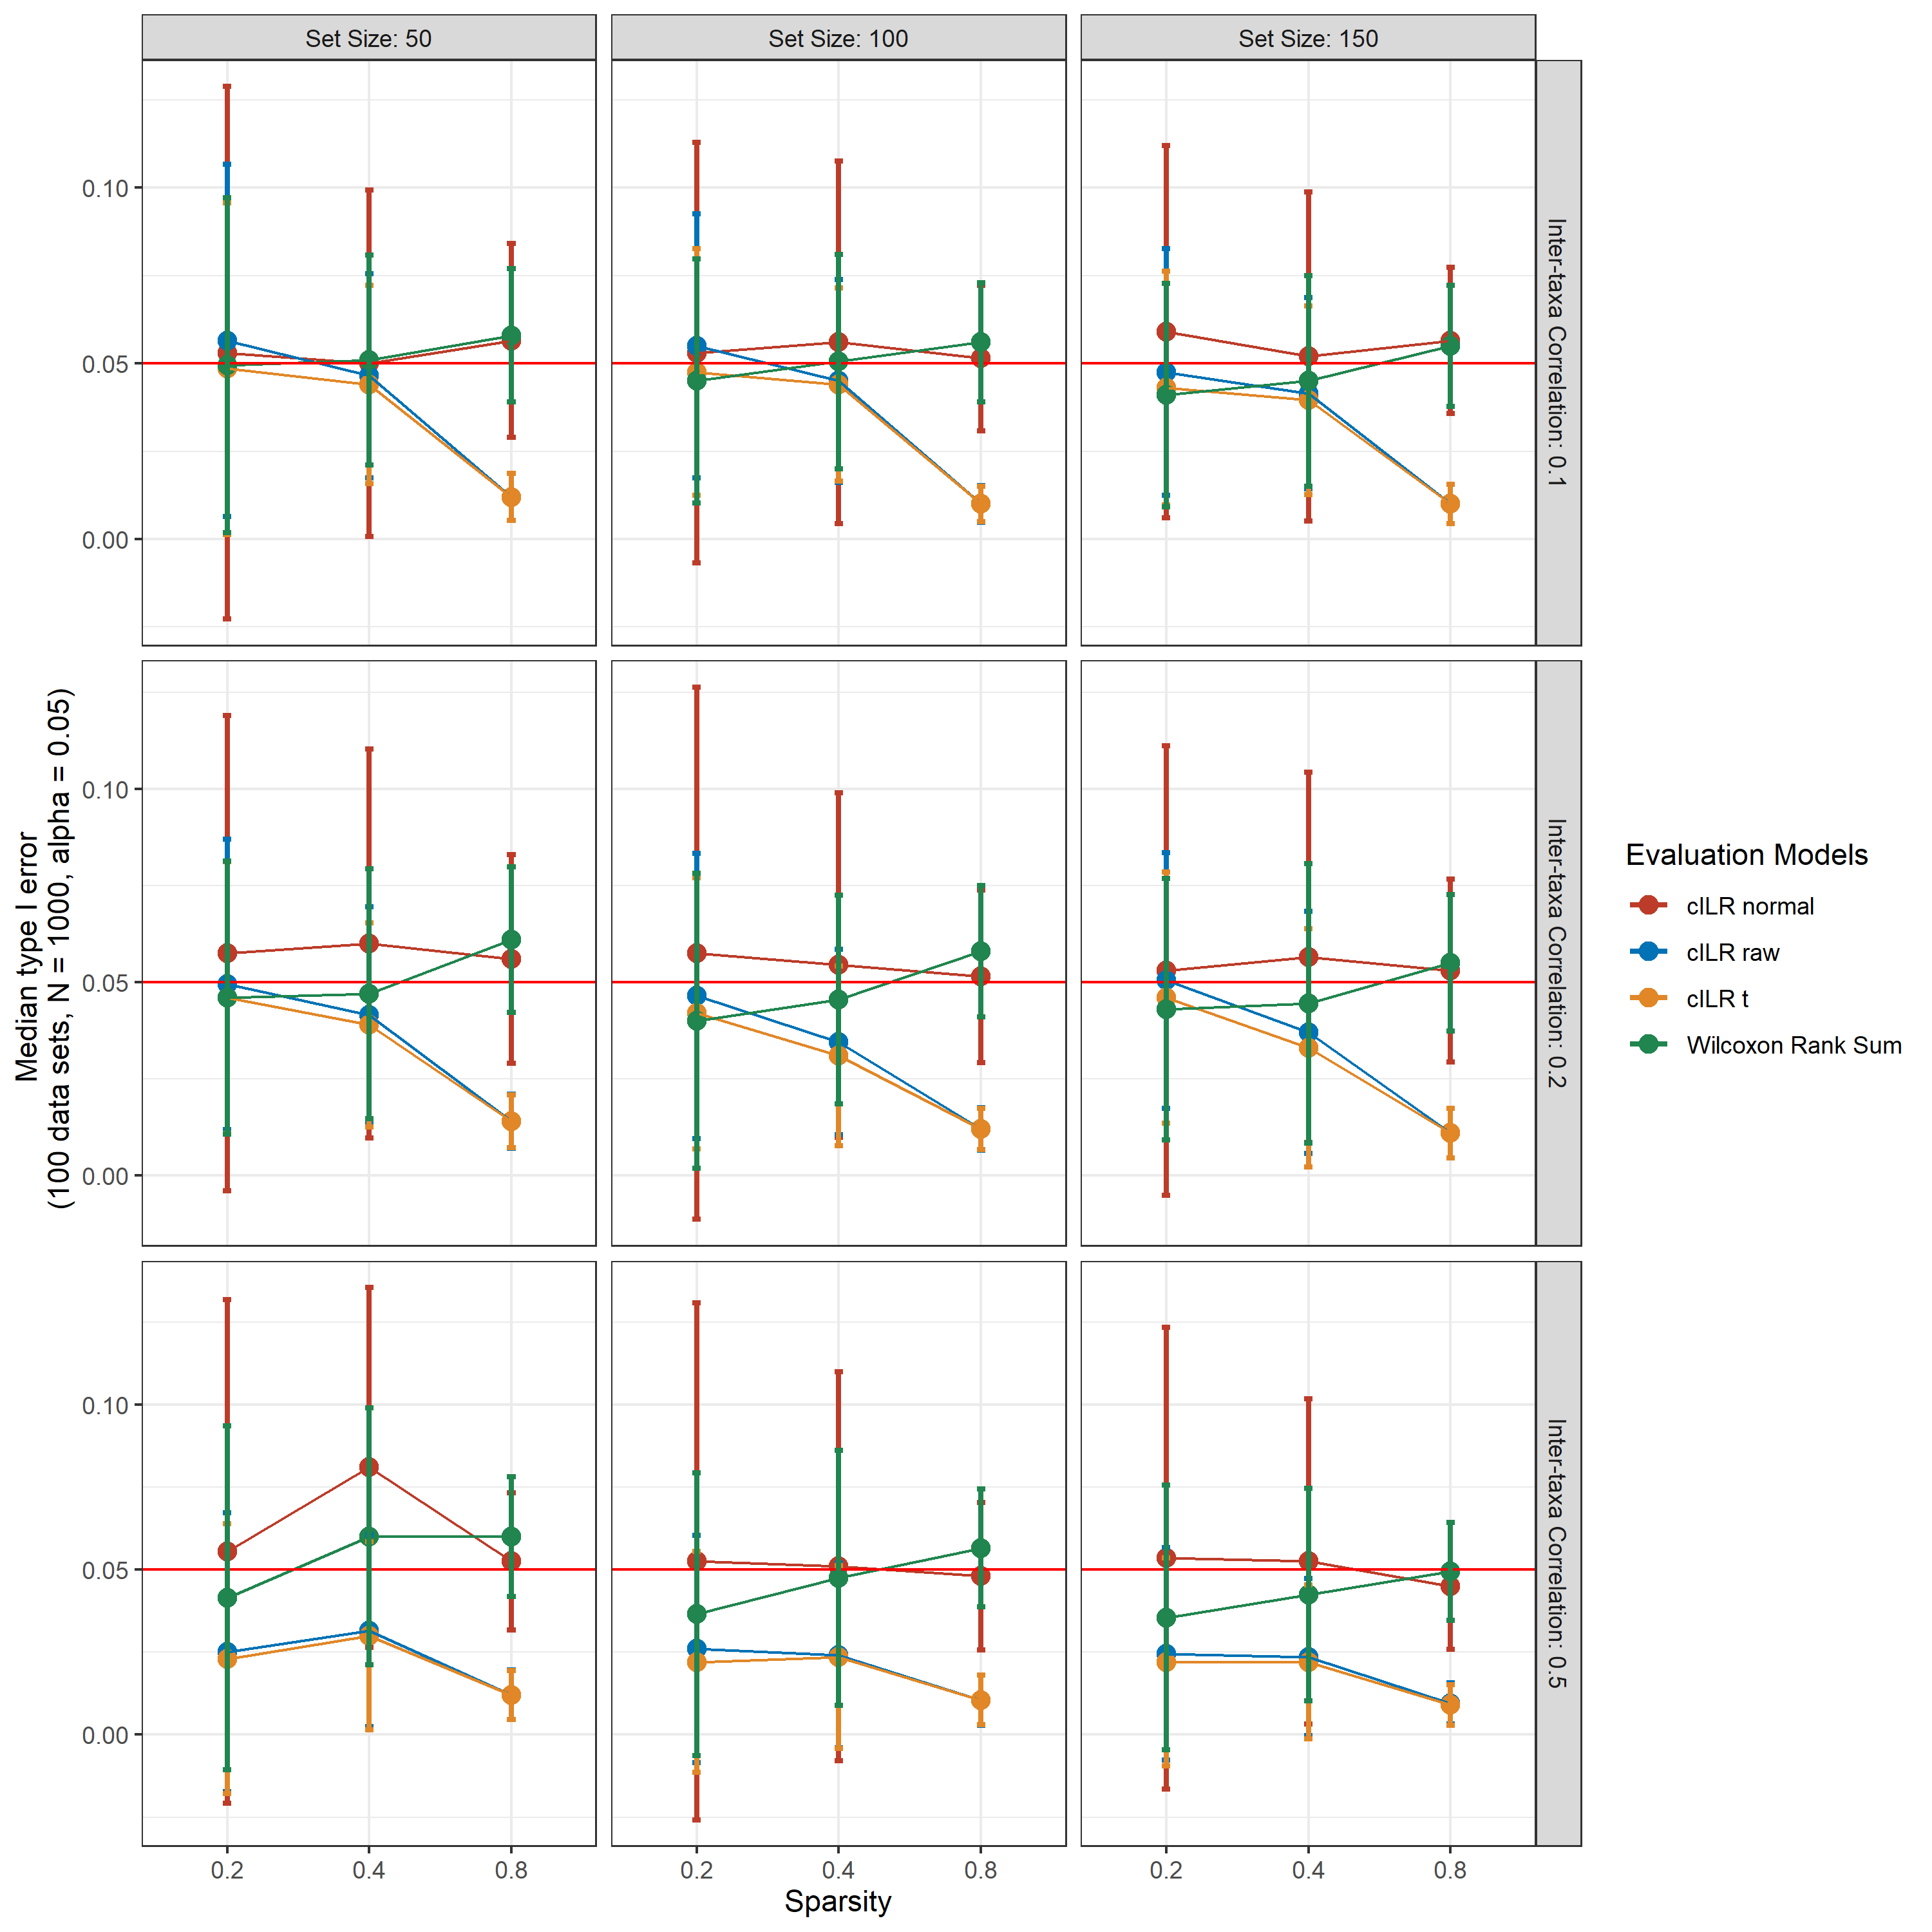
\includegraphics[scale = 0.5]{figures/fdr_single_sample.png}
    \caption{Median type I error rate as a function of data sparsity benchmarked on simulated null microbiome data as enumerated in SI methods. Enrichment of a specified set was tested at the sample level using cILR and the Wilcoxon rank sum test at $\alpha$ of 0.05. Each panel represents different in set size (horizontal) and inter-taxa correlation (vertical)}
\end{figure}

\begin{figure}[H]
    \centering
    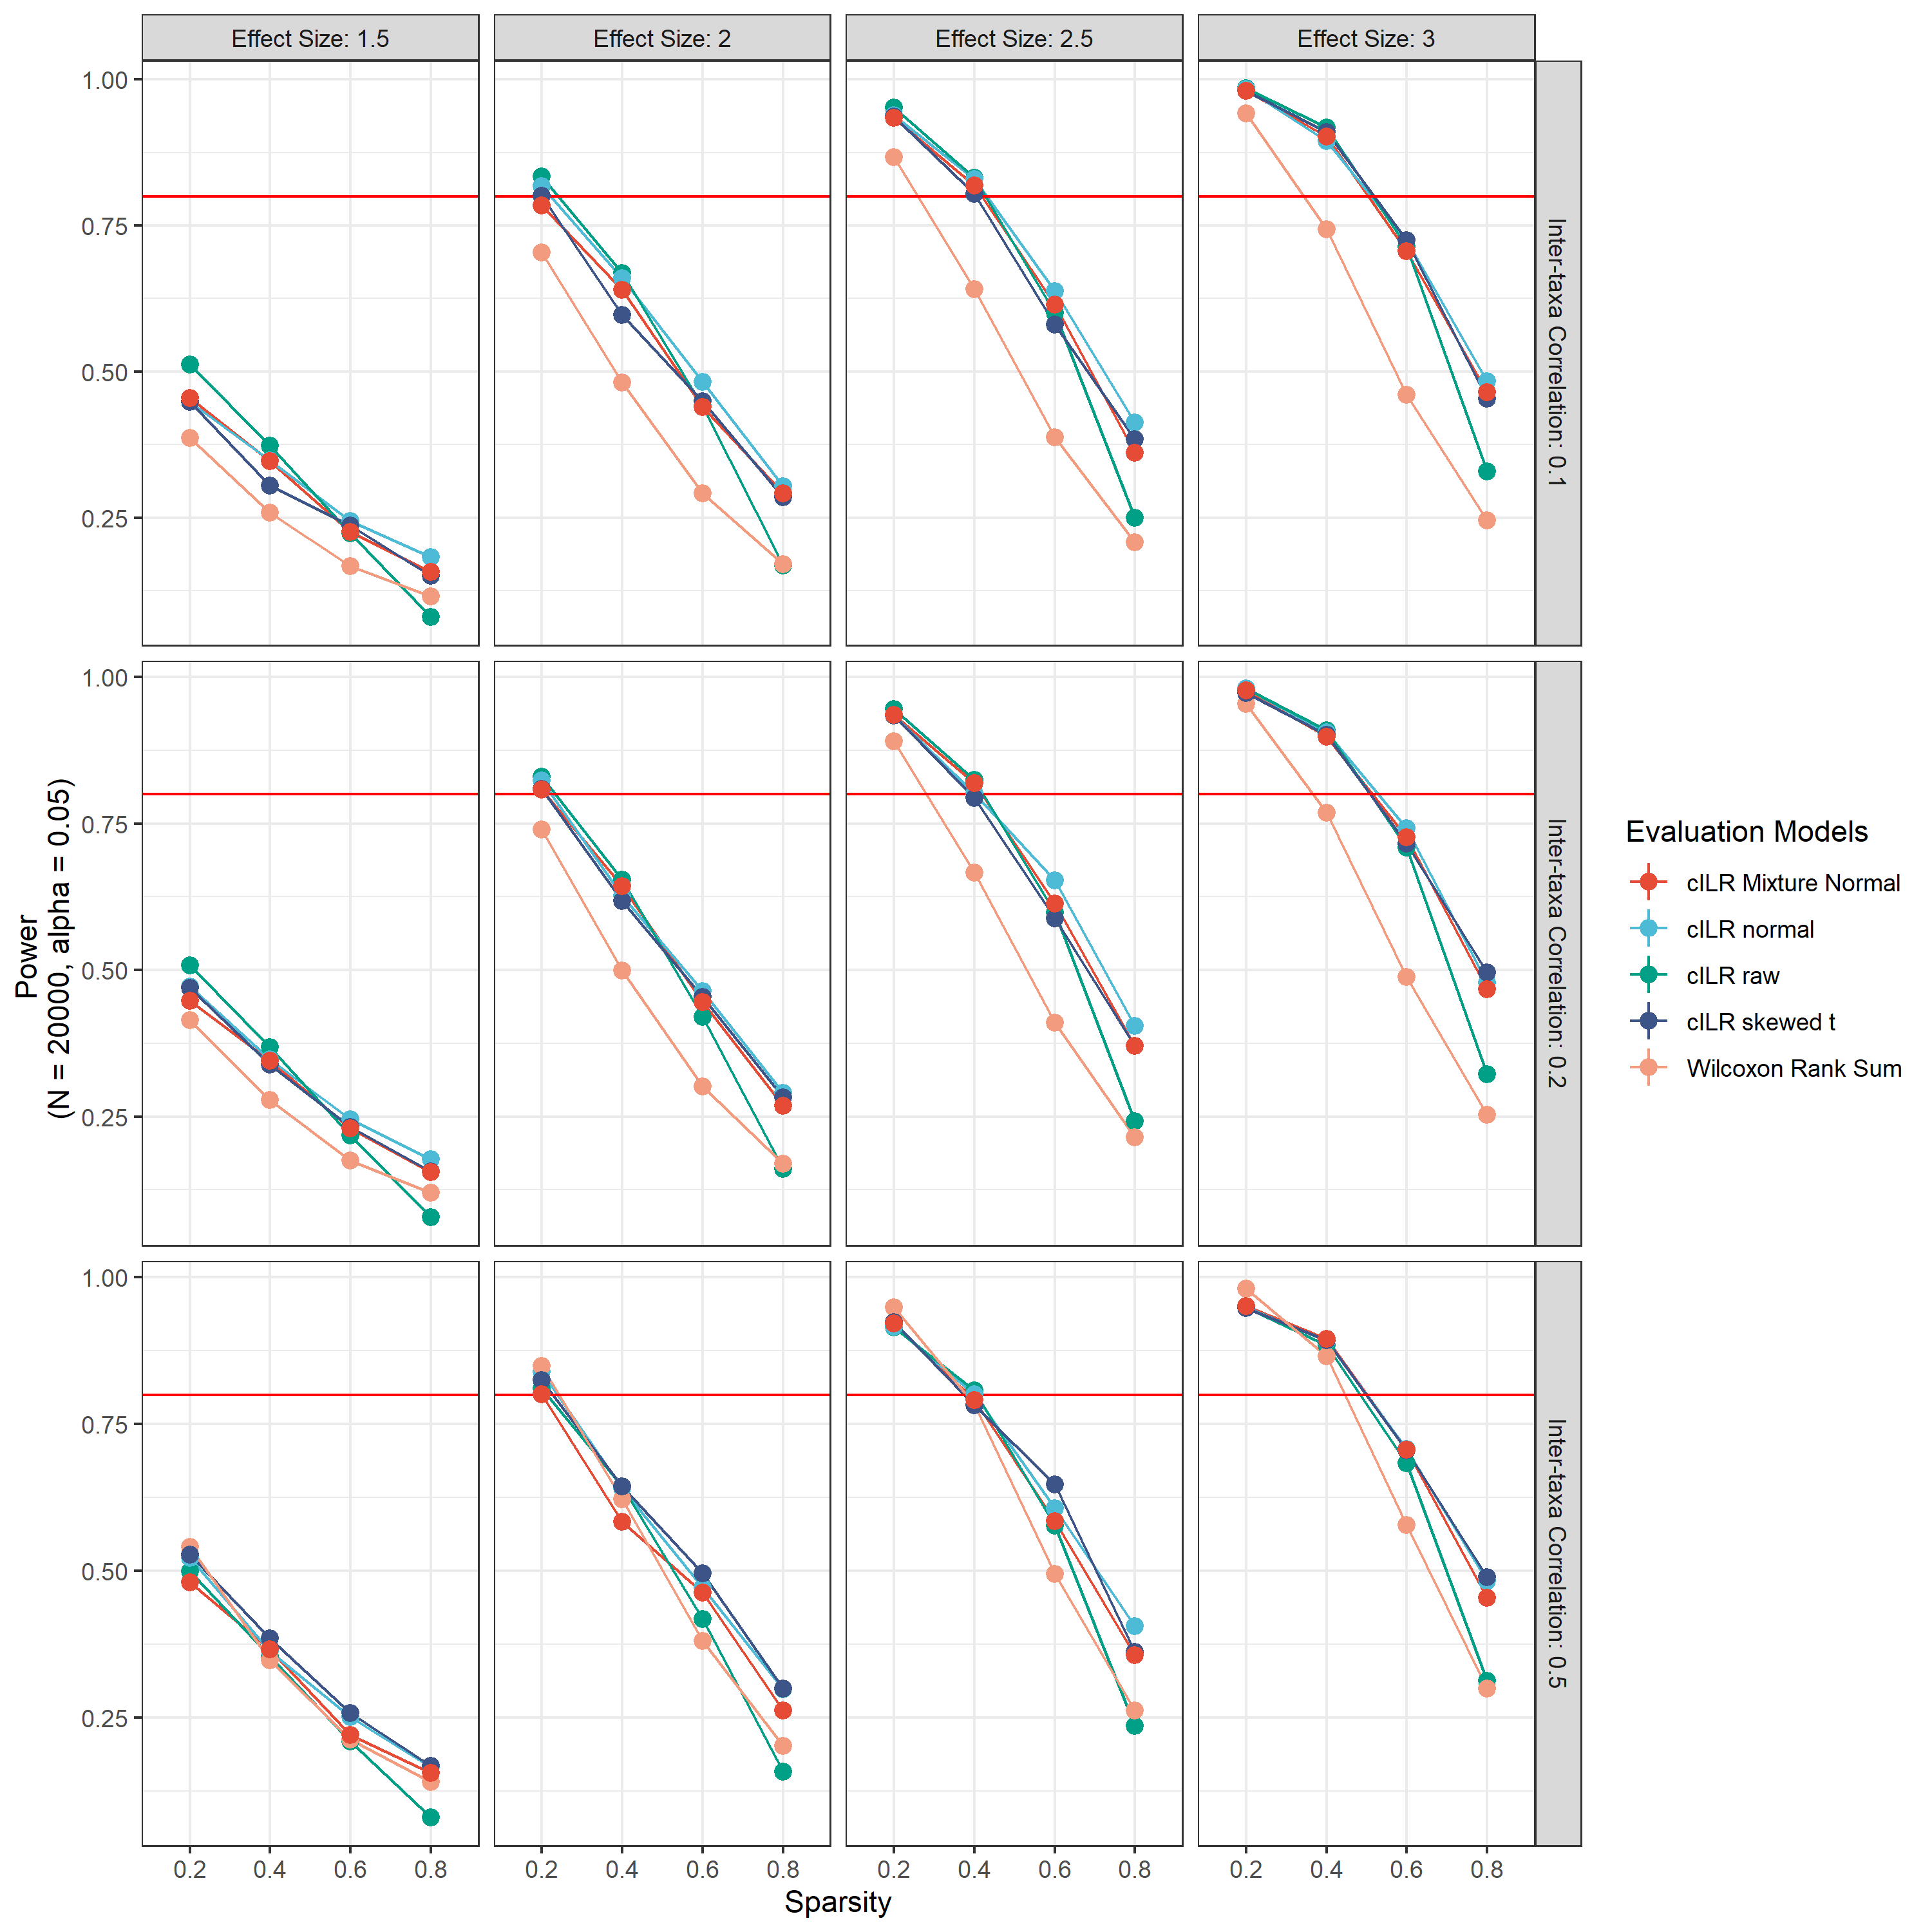
\includegraphics[scale=0.5]{figures/pwr_single_sample.png}
    \caption{Median power as a function of data sparsity benchmarked on simulated microbiome data as enumerated in SI Methods. Enrichment of a specified set was tested at the sample level using cILR and the Wilcoxon rank sum test at $\alpha$ of 0.05. Each panel represents different effect sizes (horizontal) and inter-taxa correlation (vertical).}
\end{figure}

\section*{Real data analysis} 
\subsection*{Type I error control}
We benchmark type I error rate on 16S and WGS data from the Human Microbiome Project (HMP) obtained from the packages \emph{HMP16SData} (ver. 1.9.3) and \emph{curatedMetagenomicData} packages in R. For each data set, we filtered out samples with library size less than 1000, as well as taxa with a proportion of zeroes of 0.9 or more. We then randomly assigned each sample into one of two arbitrary groups.  \\

\newpage
\bibliography{tax_agg}{}
\bibliographystyle{plain}
\end{document}
\end{document}